%Préambule du document :
\documentclass[12pt, a4paper]{book}
%\usepackage[latin1]{inputenc} 
\usepackage[utf8]{inputenc} % accents
\usepackage{gensymb} % degree symbol ° (\degree)
\usepackage[T1]{fontenc} % | "`pipe"' character
\usepackage{graphicx}
\usepackage{titling}
\usepackage{amssymb} 
\usepackage{minitoc} % chapter's tocs
\usepackage{authblk} % author affiliations
\usepackage{fancyhdr} % modify the headers
\usepackage{tabularx} % tables not larger than A4
\usepackage[table]{xcolor} %colors inside the tables
\usepackage{float}
\usepackage{multicol} % multiple columns in some sections
\usepackage[inner=2cm,outer=2cm]{geometry} %A4 margins
\usepackage{siunitx}
\usepackage[labelfont=bf, margin=0.5cm]{caption} % for figure captions in minipages
\usepackage{hyperref} %link references (toc, citations) inside document
\usepackage{natbib} % to cite with parentheses and plain text et only year if you please...
\usepackage{amsmath}
 \usepackage{fixltx2e} % allows overrightarrow to be in caption
 \MakeRobust{\overrightarrow}


\bibliographystyle{plainnat} % reference style
\renewcommand{\bibname}{References} %Rename "`bibliography"' => "`references"'
\newcommand*{\doi}[1]{\href{https://doi.org/#1}{doi: #1}}


\hypersetup{
    colorlinks,
    citecolor=brown,
    filecolor=green,
    linkcolor=red,
    urlcolor=blue
}
\hypersetup{linktocpage}


\pagestyle{fancy}
\fancyhead{}
\fancyfoot{}
\fancyhead[RO,LE]{\thepage}
\fancyhead[LO]{\leftmark}
\fancyhead[RE]{\rightmark}
\setcounter{tocdepth}{1} % we only want chapters and sections in toc
\setcounter{minitocdepth}{2} %we want sections and subsections in chapters' minitocs

\pretitle{%
  \begin{center}
  
  
\includegraphics[width=17cm]{../Logo_software.png}\\[\bigskipamount]
}
\posttitle{
\\
  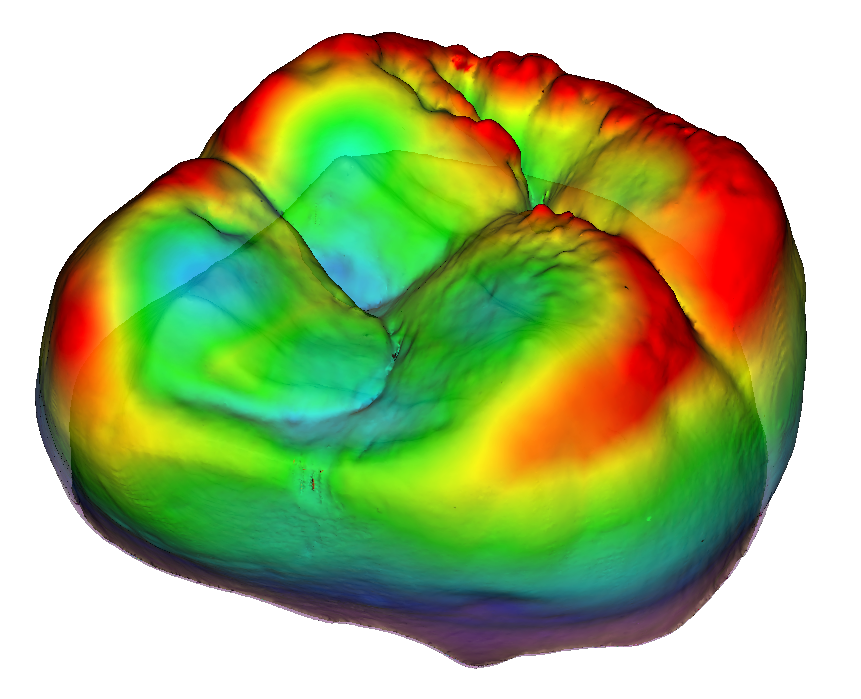
\includegraphics[width=8cm]{tutorial08.png}\\[\bigskipamount]
\end{center}}

%\postdate{
%
\includegraphics[width=15cm]{logo_affiliations.png}
%}

\title{Tutorial 08: thickness between objects}



%\titlepicture[width=13cm]{Logo_software.png}
\author{Renaud LEBRUN}
\affil{Institut des Sciences de l'Evolution, Université de Montpellier, France}
\date{\today} 

\def\chaptername{Tutorial}
\setcounter{chapter}{8}
%Corps du document :
\begin{document}

	\dominitoc

\maketitle


\faketableofcontents

%\chapter{Working with landmarks}
\addstarredchapter{Thickness between objects}

\markboth{Tutorial 08: thickness between objects}{}

\minitoc 
Tutorial 08 includes:
\begin{itemize}
\item One .ntw (MorphoDig project) file
\item Two .vtk surface files representing the Enamel Dentine Junction (EDJ) and Outer Enamel Surface (OES) of a Neolithic human upper left second molar.
\item Two .pos (position) files 
\item The present .pdf document
\end{itemize}



\section{About the specimen}
The 3D model corresponds to a virtually reconstructed crown of a left upper permanent second molars (LUM2) from a Neolithic human of the necropolis of Gurgy (France). This specimen (GLN04-201-ULM2) was published in \citet{LeLuyer2016}, and the 3D model was released in \citet{LeLuyer2016a}.
The 3D data were obtained by computerized microtomography at the MRI \si{\micro}CT platform housed at the ISEM. 


\section{A brief overview of enclosed files}
		
The present tutorial contains a project .ntw file, which is useful to open the two surfaces in convenient positions. Open the enclosed .ntw file (File->Open Project, then select "Enamel\_thickness.ntw"). Once loaded, the two surfaces are opened, are given the positions enclosed in the two position files, and a color. Note that the newly opened surfaces are unselected.


\section{Tutorial}

\subsection{Thickness between objects}
The OES (Outer Enamel Surface) 3D representation already contains a "Thickness" scalar array. This thickness was produced as follows (see also Fig. \ref{thickness_between}, p.\pageref{thickness_between}): \\
1) The two surfaces were loaded, and the "Compute thickness between two surfaces" dialog was opened (Scalars->Compute thickness between two surfaces). It does not matter here whether these two surfaces are selected or not.\\
2) The Maximal thickness was set to "3mm", as we do not expect enamel thickness to exceed 3mm within this tooth. Note that in order to minimize computation time, this value should be set as low as possible. We could have chosen a larger value, which would lead to the same result but would take a significantly larger amount of time.\\
3) The "use neighbour vertices to smooth search direction" checkbox was checked, in order to produce a smoother output. \\
4) \textbf{Most important parameter}: the "invert normals of observed object" checkbox was checked, as the thickness computation process expects the normals of the observed object (here, the EDJ) to be in the opposite direction as those of the impacted object (here the EOS) \\

\begin{figure}
  \centering
  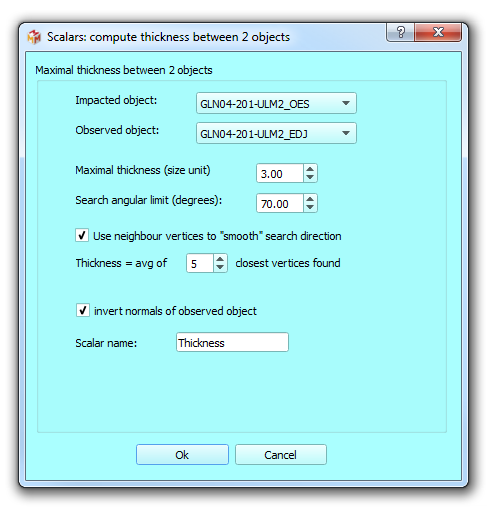
\includegraphics[scale=0.5]{thickness_between.png}
\caption{Enamel thickness computation. The impacted object is the Outer Enamel Surface. The observed object is the Enamel Dentine Junction (EDJ). Maximal thickness was set to "3", because we do not expect enamel thickness to exceed 3mm. The "use neighbour vertices to smooth search direction" checkbox was checked. \textbf{Most important parameter}: the normals of the observed object (EDJ) where inverted, as we expect the normals of the Impacted and Observed objects to be in opposite directions.}	
\label{thickness_between}
 \end{figure}

The result of thickness computation is illustrated in Fig. \ref{thickness_colormap}, p.\pageref{thickness_colormap}. 

\begin{figure}
  \centering
  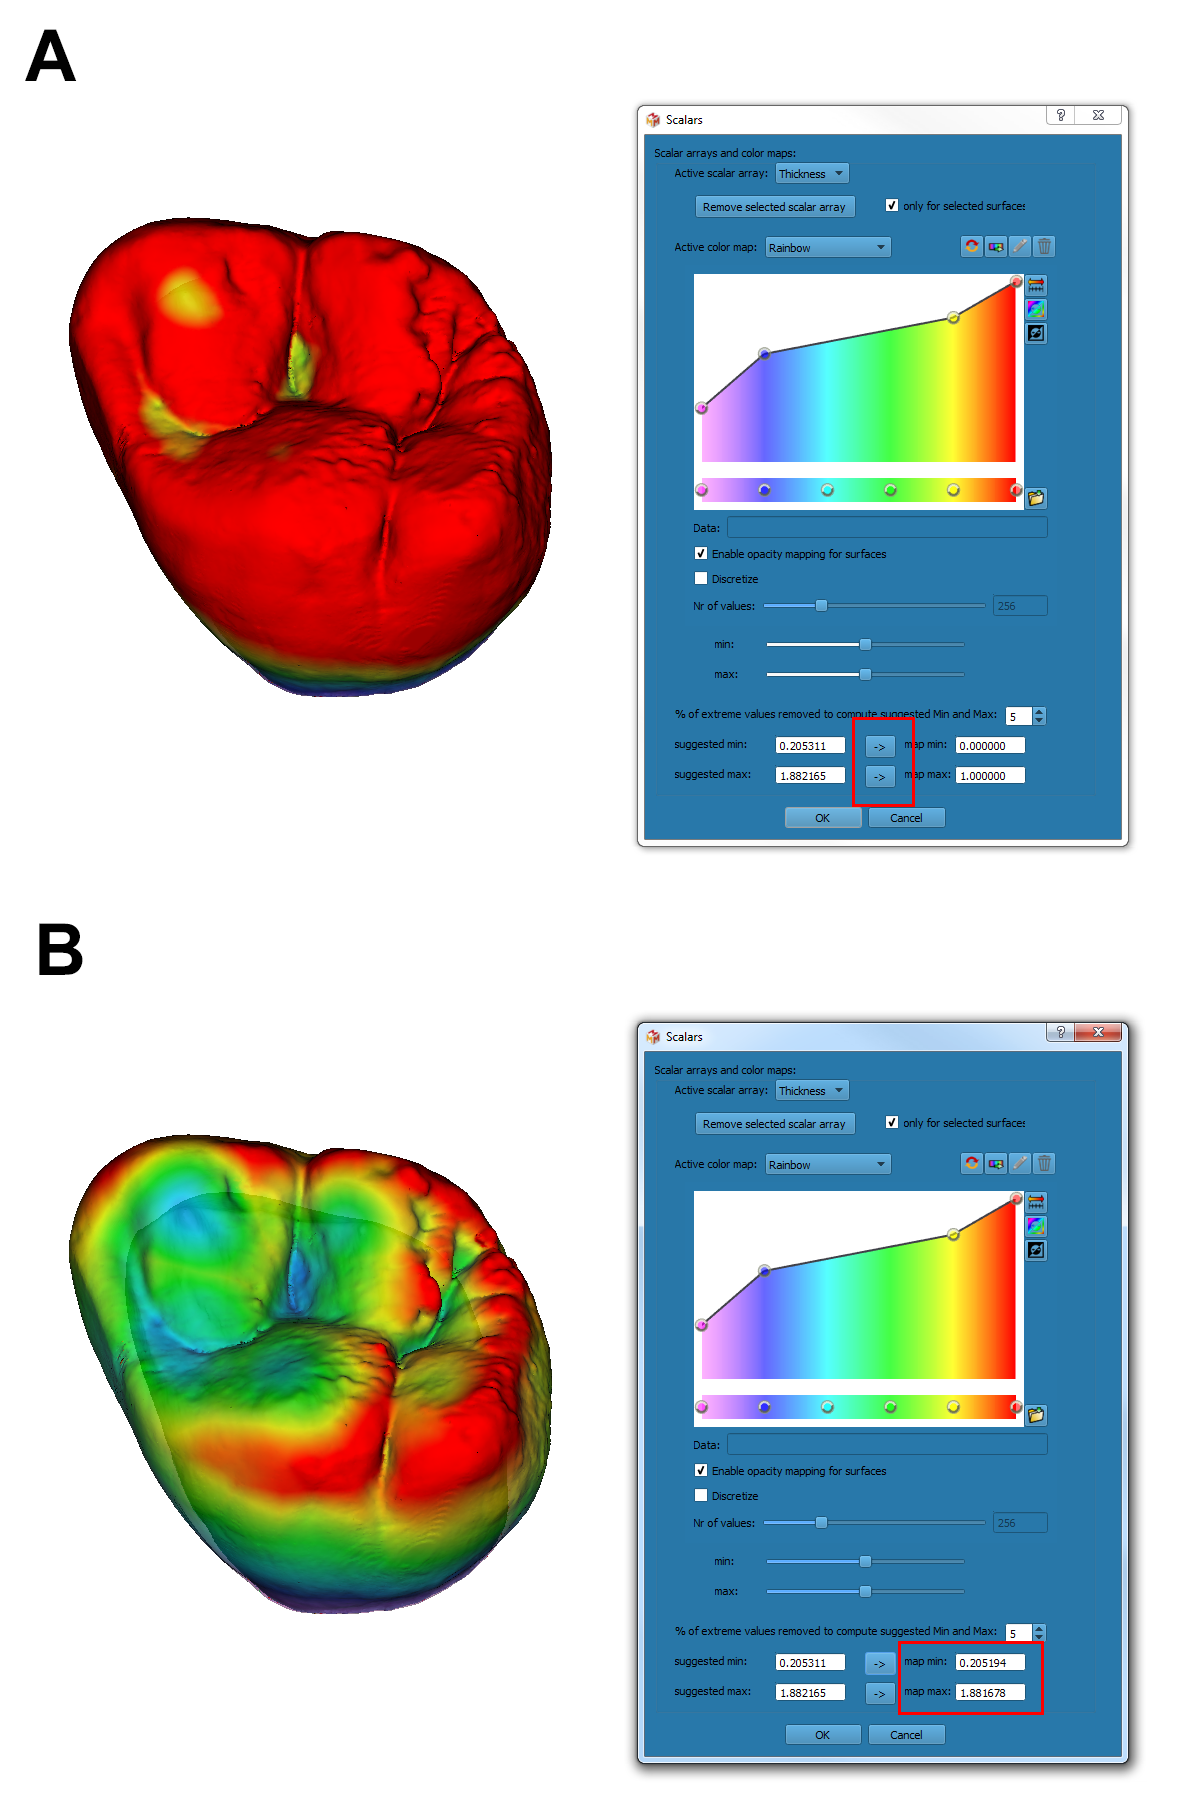
\includegraphics[scale=0.33]{thickness_colormap.png}
\caption{Enamel thickness distribution in a left upper second molas of \textit{Homo sapiens}. \textbf{A:} The color map is by default set to range between 0 and 1 (right), which makes it uneasy to see enamel thickness variation, as enamel thickness is greater than 1mm in most regions. \textbf{B:} The color map was adjusted to range beteen around 0.2 mm and 1.9 mm (right), which makes it easier to visualize enamel thickness variation.}	
\label{thickness_colormap}
 \end{figure}

\section{Acknowledgements}
MicroCT data acquisition was funded by the Research National Agency through the DHP project (dir: S. Rottier; 2012-14; Université Bordeaux 1/LaScArBx; Grant number: ANR-10-LABX-52) and the PEPS 3Dent’in (dir: P. Bayle; 2013-14; PEPS IdEx Bordeaux/CNRS; Grant number: ANR-10-IDEX-03-02). M. Le Luyer, who performed 3D data acquisition, benefited from a doctoral grant of the Ministère de l’Enseignement Supérieur et de la Recherche. MicroCT data presented in this work were produced through the technical facilities of the MRI platform and of the labEx CeMEB.


%\nocite{*}   % All bibliography items appear without citation in the text

%\cleardoublepage
%\phantomsection

\addcontentsline{toc}{section}{References}
\bibliography{References}	

\end{document} 

